\chapter{Results and Discussion}
The results presented here concern the solution of the adiabatic equation, i.e. the adiabatic potential curves $U_{\nu}(\rho)$. The potential adiabatic potential curves $U_{\nu}(\rho)$ were obtained by numerically solving  \eqref{adiabatic} using the method described in \cref{chapter:5}. 

Note the similarities of the 

Signatures of the Efimov effect can be revealed by analyzing the structure of the adiabatic hyperspherical potentials. In the scale free region $r_l \ll \rho \ll
\abs{a}$ the lowest adiabatic hyperspherical potential becomes attractive and proportional to $\rho^{-2}$ this emerging attractive effective potential   For $a<0$ Efimov states are expected to emerge from the three atom contiuum. This can be seen in \Cref{fig:res_3} where the lowest continuum curve. However, for $a>0$ Efimov states will emerge from the atom-diatom threshold      
 
$ E = 0$ is the dissociation limit
for three free particles, while $E < 0$ dissociation limit represents one bound two-body state plus a free particle.
 
 Efimov physics comes into play in the intermediate region $r_0 \ll \rho \ll \abs{a}$. In this region, the effective potentials are still proportional to $\rho^{-2}$ but modifictations of $W_{\nu}$ leads to both attractive and repulsive effective three-body potentials.   

\begin{table}[h!]
	\centering
	\begin{tabular}{||c c c c c c||} 
		\hline
		$N_{\theta}$ & $\lambda_{0 0}$ & $\lambda_{1 3}$ & $\lambda_{2 6}$ & array(s) & dsygvd(s)
		\\ [0.5ex] 
		\hline\hline
		5	   & 0.000 000 000 0214   & 32.000 000 071 3015 & 60.000 002 031 0135 & 0.66 & 0.00  \\
		10     & -0.000 000 000 0417  & 32.000 000 000 1003 & 60.000 000 000 2154  & 4.58 & 0.00 \\
		15 & 0.000 000 000 0007 & 32.000 000 000 1309 & 59.999 999 999 8871& 12.32& 0.02 \\  [1ex] 
		\hline
	\end{tabular}
	\caption{Numerically calculated eigenvalues}
	\label{table:2}
\end{table}


\begin{figure}
	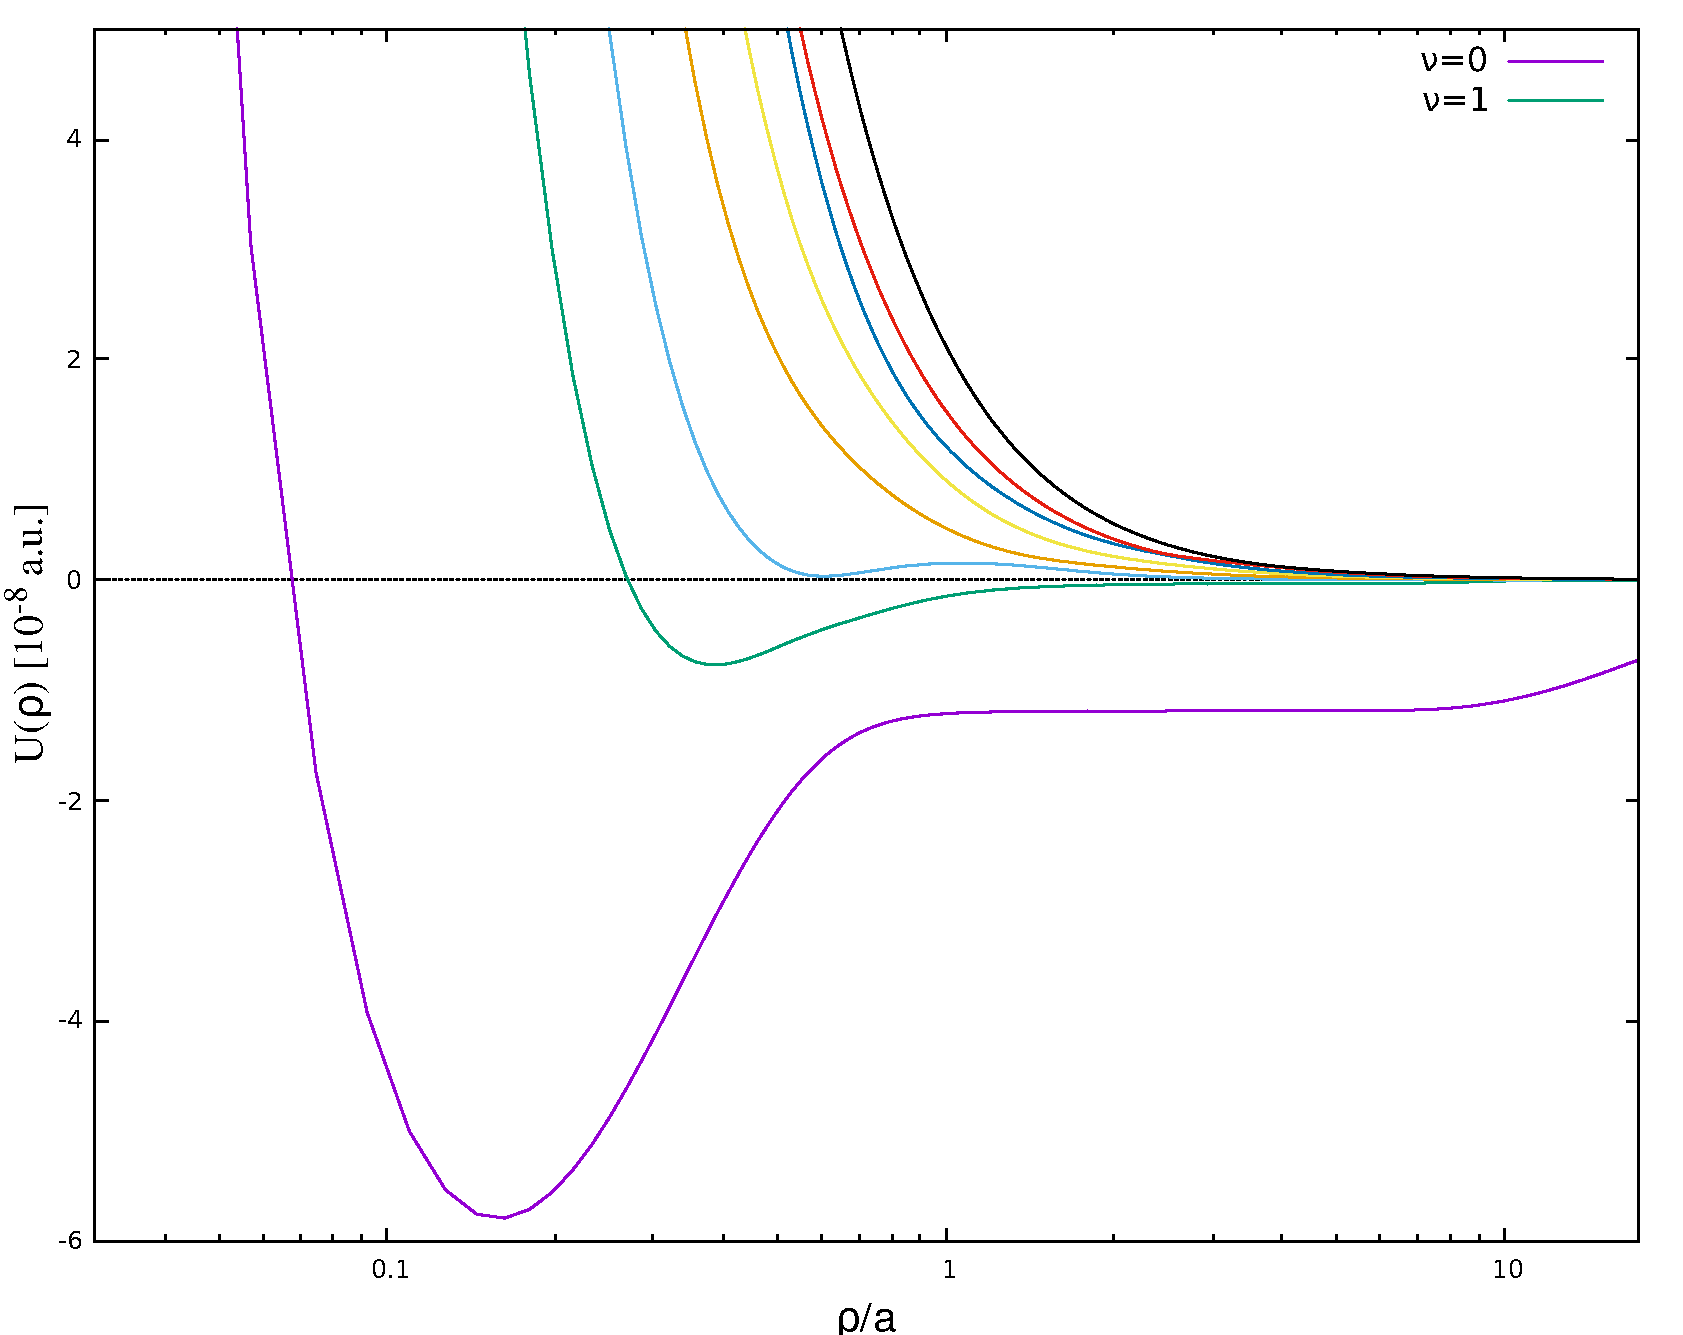
\includegraphics[width=\linewidth]{adiabatic.pdf}
	\caption{Adiabatic potential curves $U_{\nu}$ as a function of the hyperradius $\rho$ for $a=228 $ .}
	\label{fig:res_2}
\end{figure}

\begin{figure}
	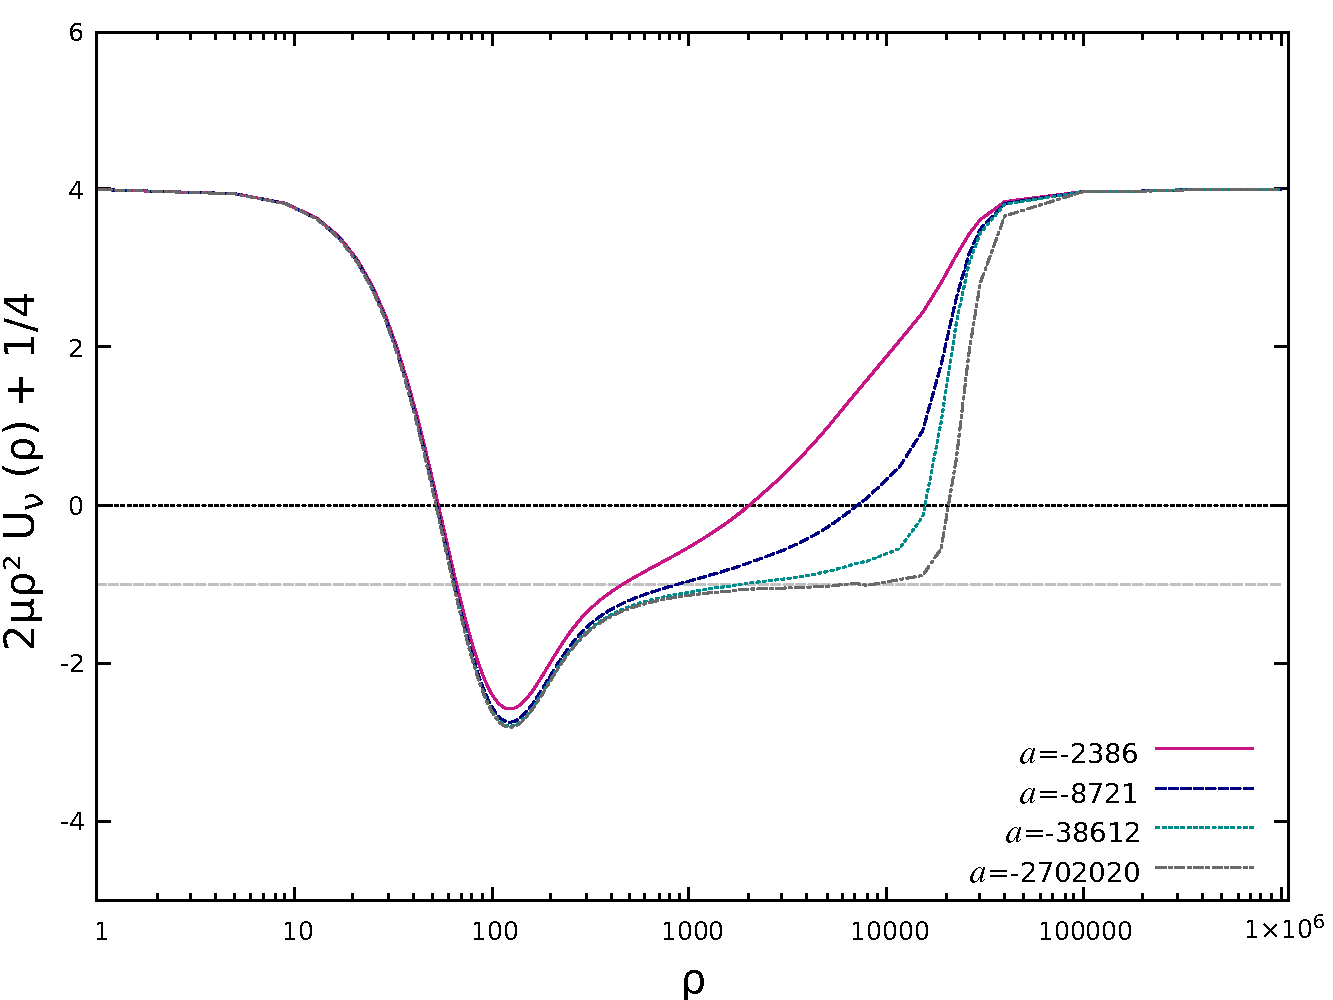
\includegraphics[width=\linewidth]{plotneg_dashed.pdf}
	\caption{..}
	\label{fig:res_3}
\end{figure}

\begin{figure}
	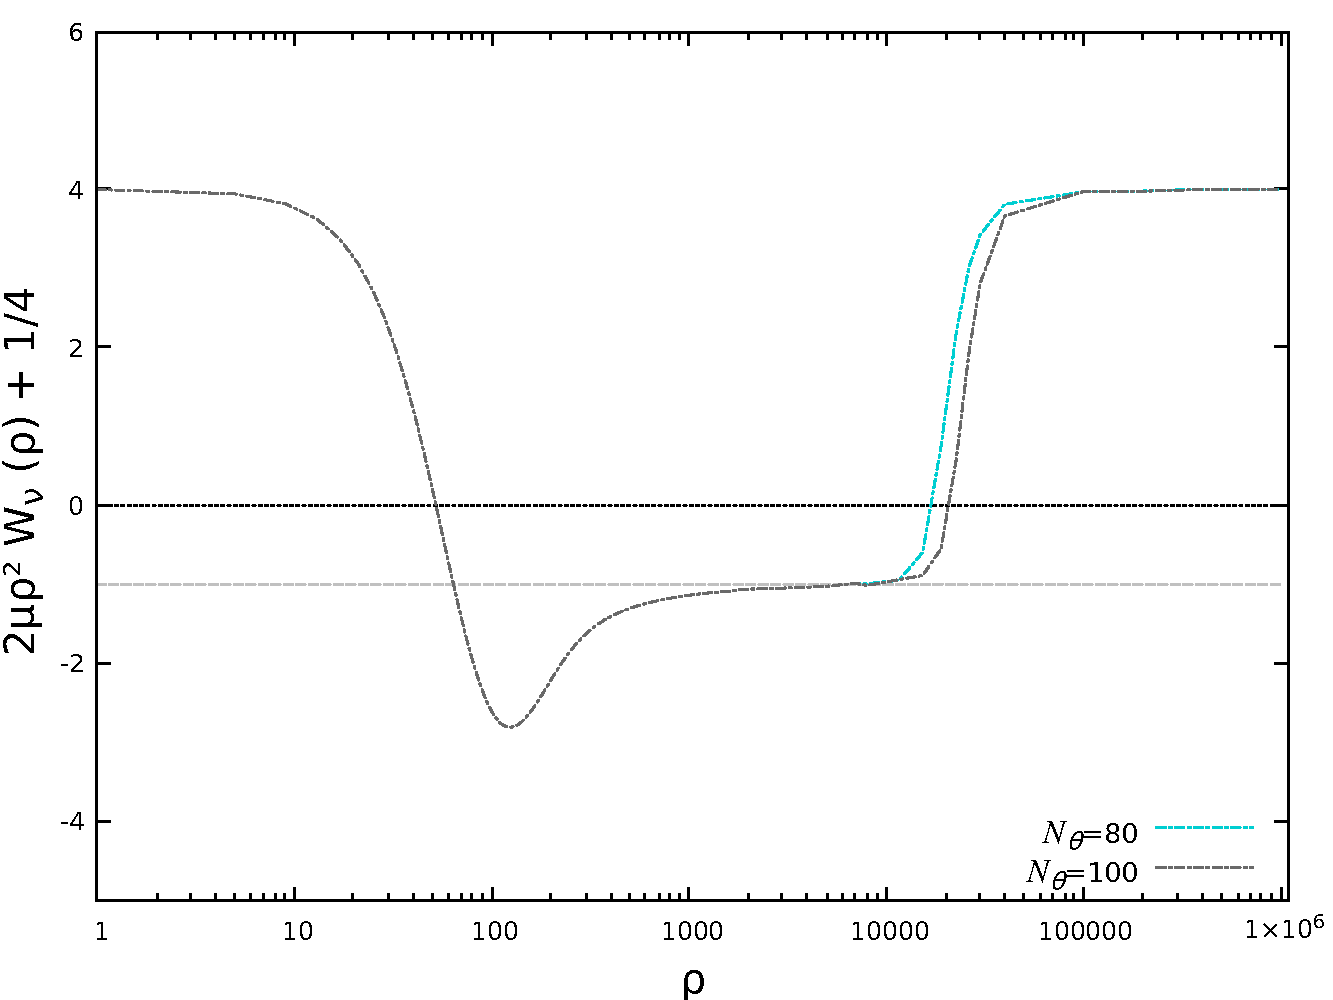
\includegraphics[width=\linewidth]{diff.pdf}
	\caption{..}
	\label{fig:res_4}
\end{figure}

\begin{figure}
	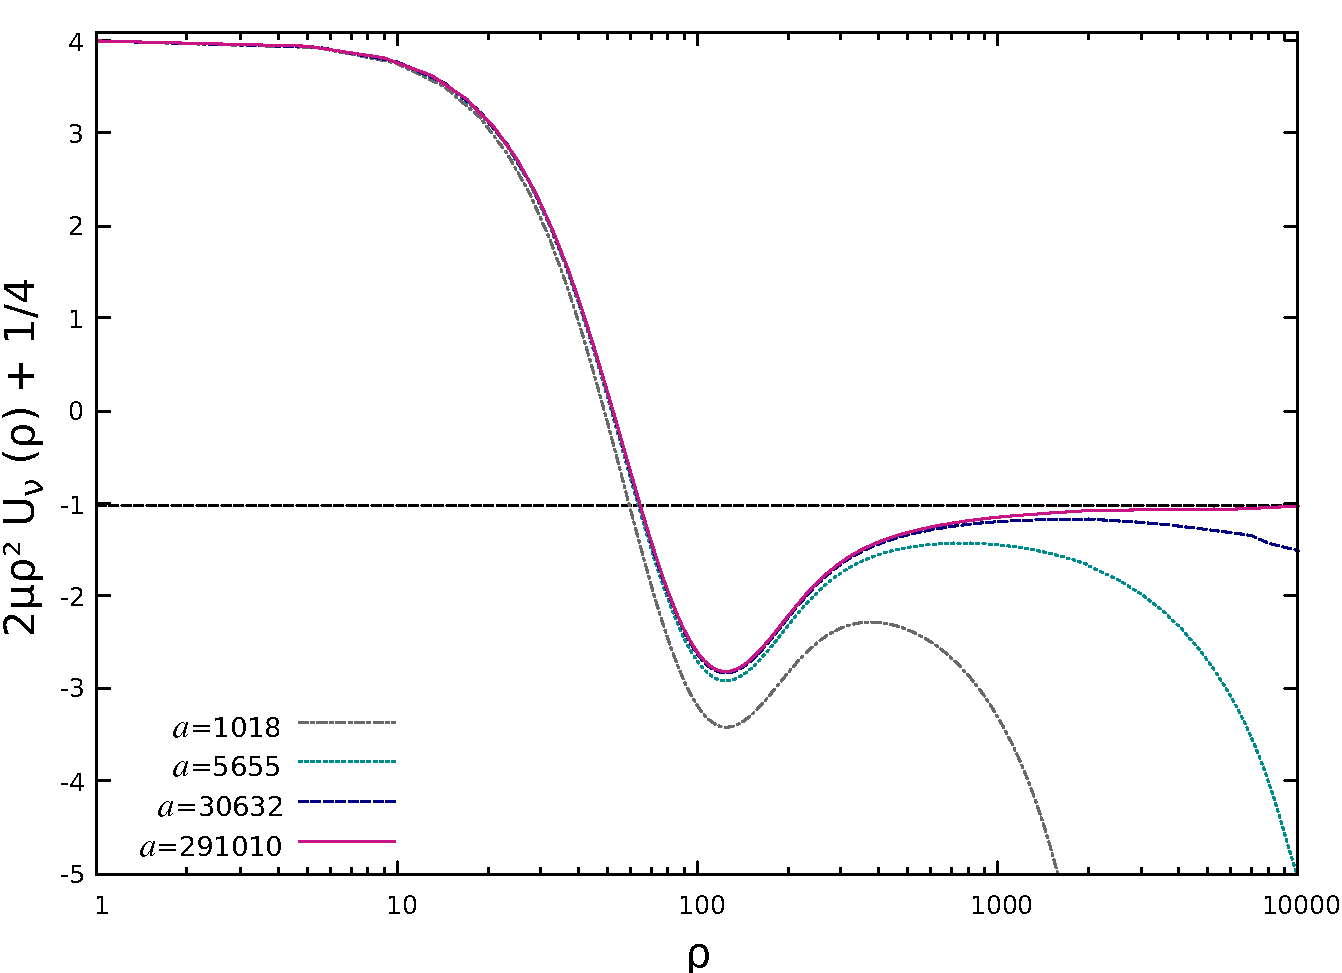
\includegraphics[width=\linewidth]{plotpos.pdf}
	\caption{..}
	\label{fig:res_5}
\end{figure}

\begin{figure}
	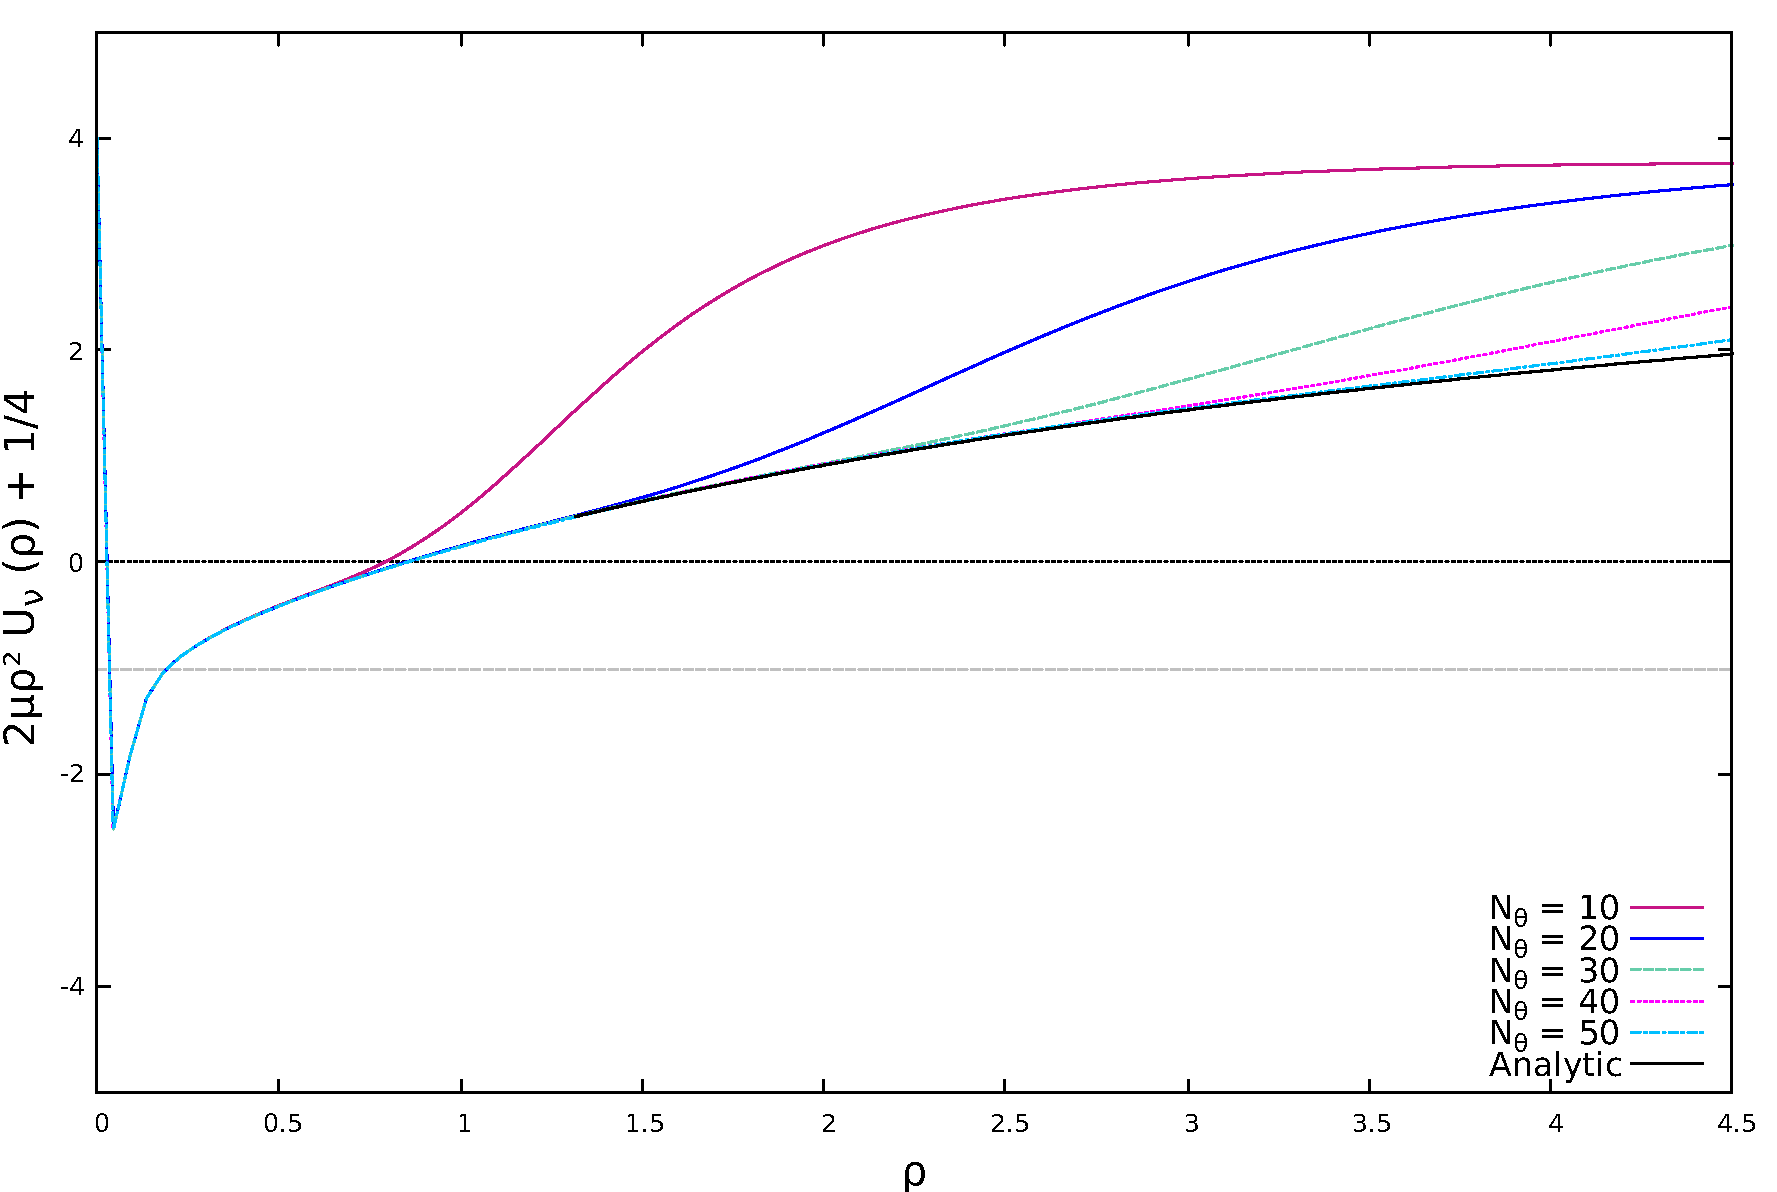
\includegraphics[width=\linewidth]{sn2385.pdf}
	\caption{..}
	\label{fig:res_6}
\end{figure}

\begin{figure}
	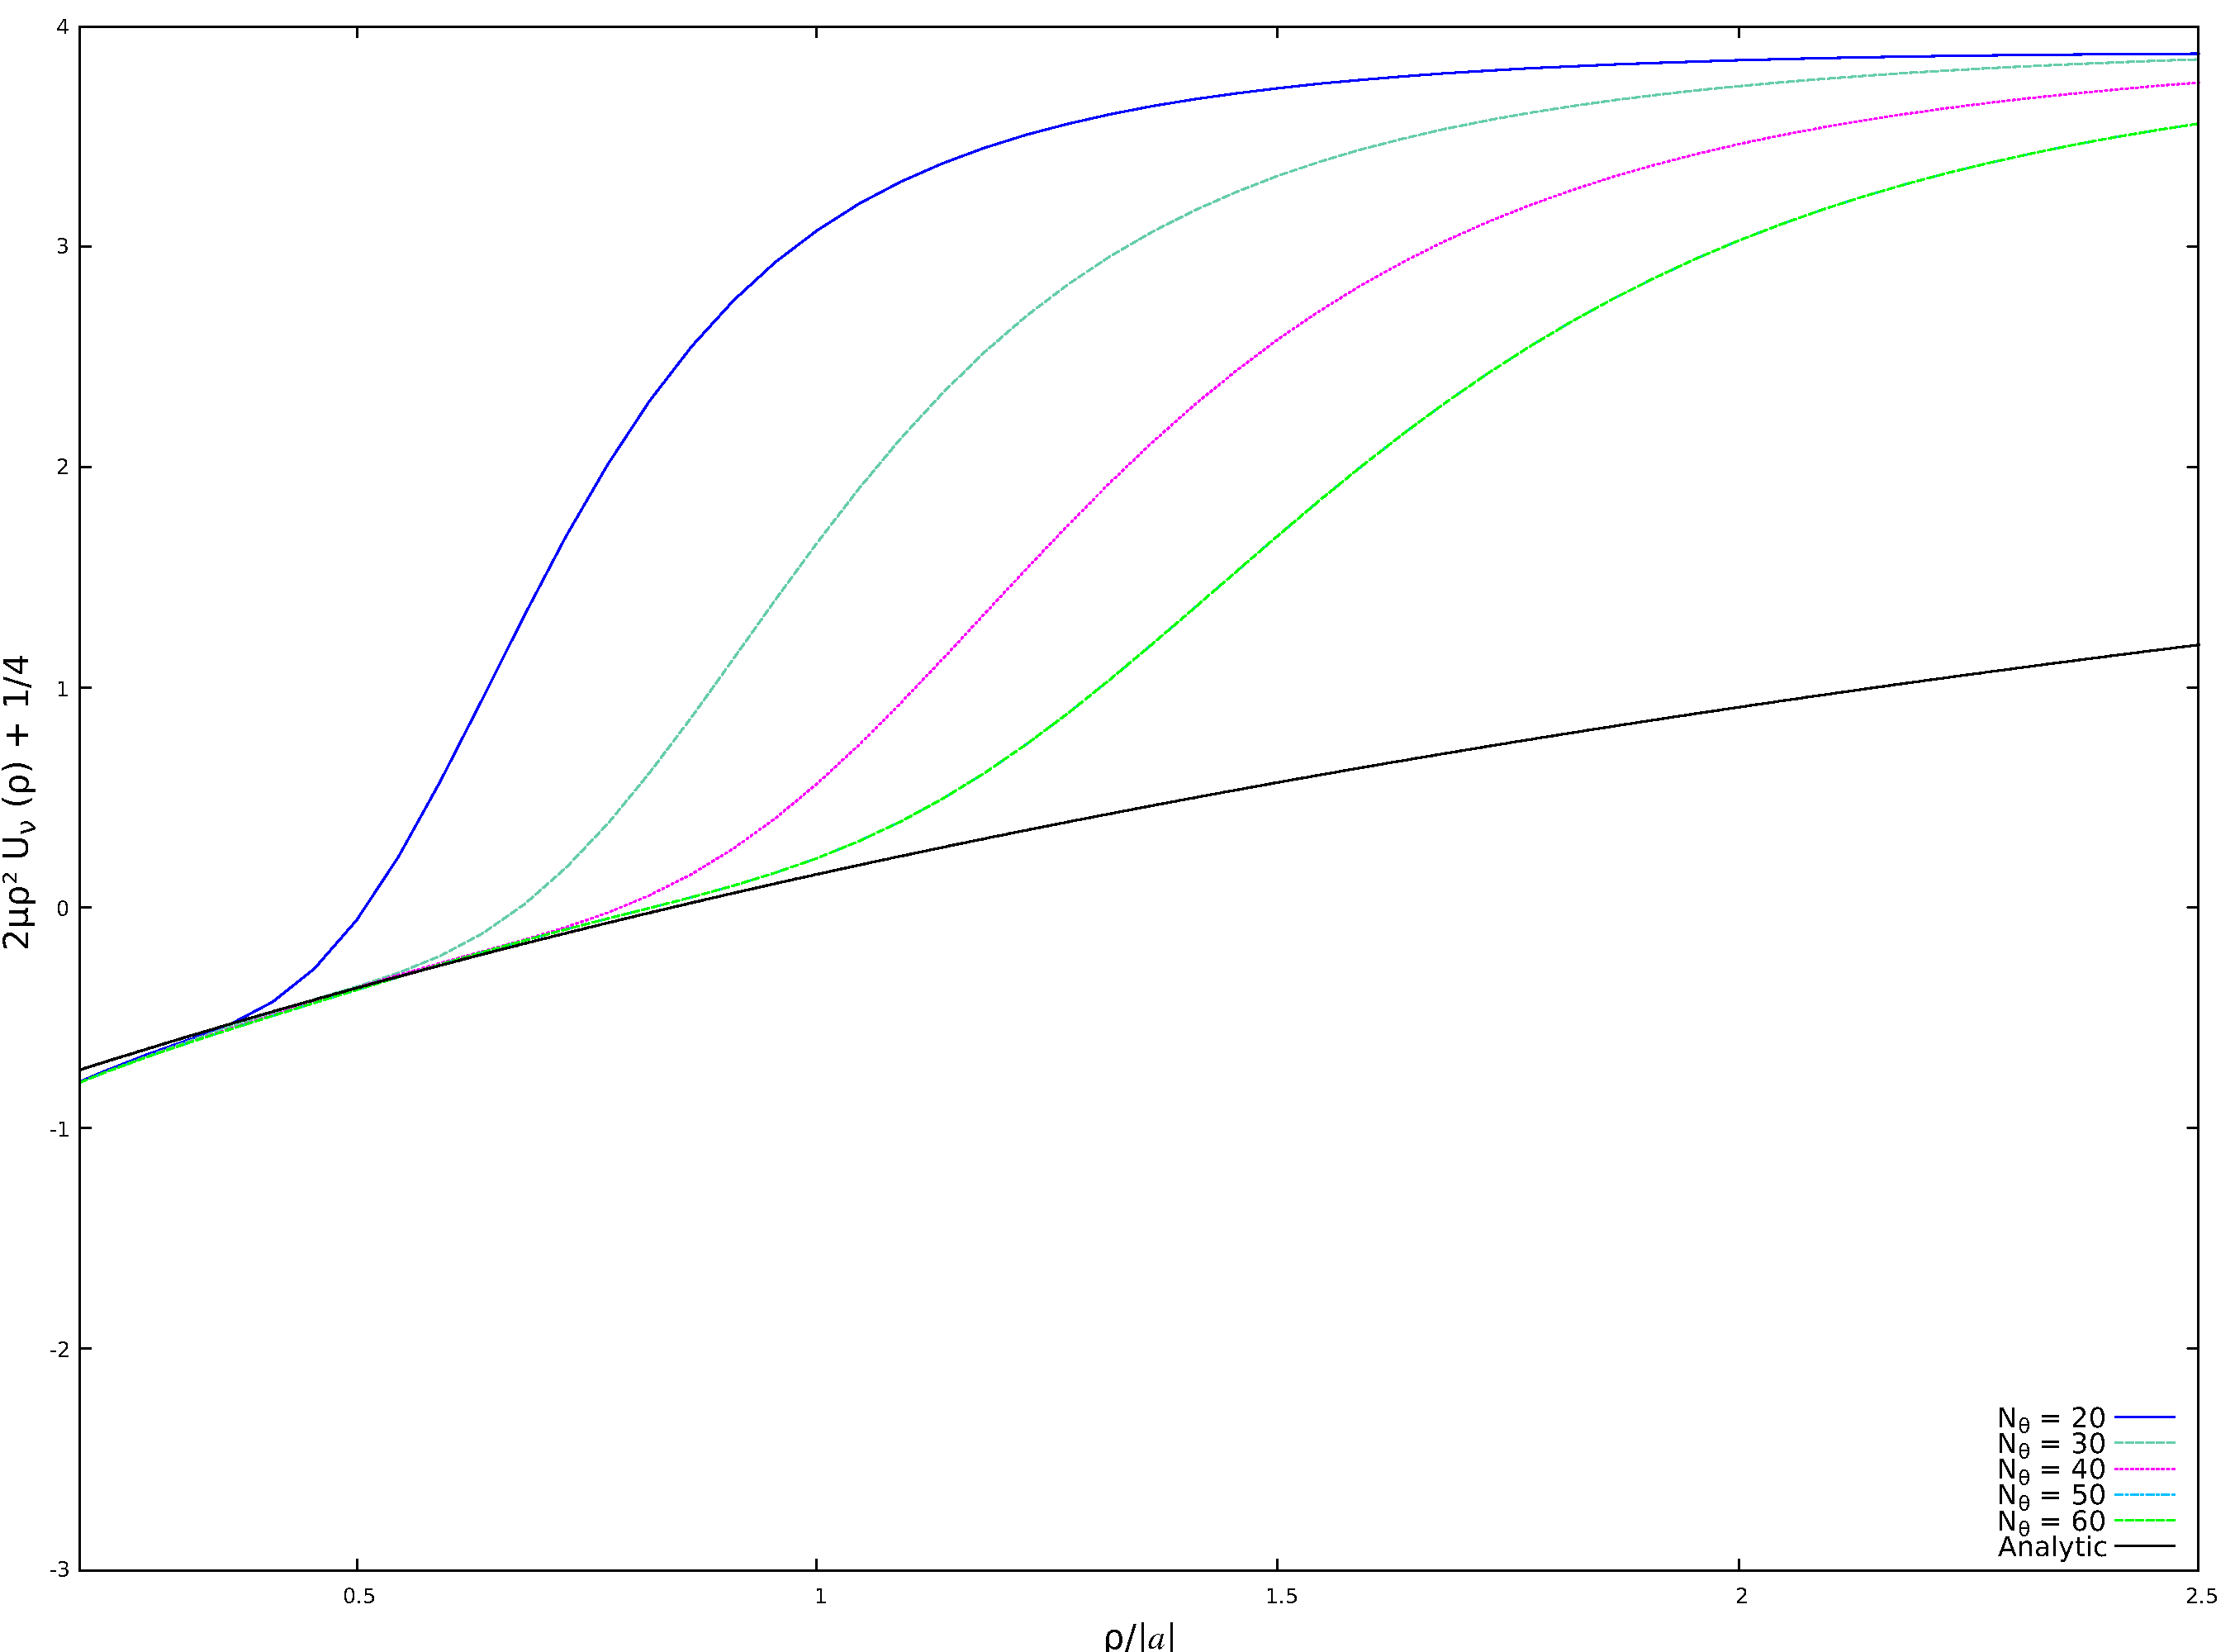
\includegraphics[width=\linewidth]{sn8720.pdf}
	\caption{..}
	\label{fig:res_7}
\end{figure}

\begin{table}[h!]
	\centering
	\begin{tabular}{||c c c||} 
		\hline
		$\rho$ (a.u.) & $N_{\theta}=80$ & $N_{\theta}=100$  \\ [0.5ex] 
		\hline\hline
		8000.0000   & -0.99789324     & -1.01719329  \\ 
		11666.667	 & -0.95232026   & -0.94496812  \\
		15333.333   & -0.59895416  & -0.89254945  \\
		19000.000   & 0.74835108  & -0.55523871   \\
		22666.667   & 2.18632828  & 0.58183597   \\
		26333.333   & 3.01480706  & 1.92849296  \\  
		30000.000   & 3.42706459 & 2.81309001  \\ [1ex] 
		\hline
	\end{tabular}
	\caption{$a = -2702020$}
	\label{table:Res_1}
\end{table} 